\subsection{Explicación formal del problema}

El problema dado se puede modelar como un grafo (no dirigido) en el cual cada v\'ertice es un planeta y las aristas representan las rutas entre los mismos, estas tienen pesos asignados los cuales representan la cantidad de litros que requieren para ser recorridas. Como se aclara que se puede llegar de un planeta a cualquier otro, podemos asumir que el grafo es conexo.

El objetivo es, a partir de un nodo 0, visitar todos los demás gastando la menor cantidad de litros posible. Esta idea de visitar todos los v\'ertices del grafo y al mismo tiempo gastar la menor cantidad de litros se puede traducir a buscar un subgrafo de ciertas particularidades, entre otras cosas que comparta los mismos nodos que el grafo original pero sacando las aristas que no valgan la pena recorrer porque podemos atravesar otras menos costosas, pero de esto hablaremos en mas detalle en la siguiente parte del informe, por ahora veamos algunos ejemplos de soluciones validas e invalidas.

Dado el el grafo de la figura (\ref{minipage:ej21}), el nodo 0 es el inicial y debemos visitar todos los demás.

\begin{figure}[H]
\centering
\begin{minipage}[b]{0.4\textwidth}
\centering
%
\begin{tikzpicture}[>=stealth',shorten >=1pt,auto,node distance=2.8cm,
                    semithick]
  \tikzstyle{every state}=[fill=red,draw=none,text=white]

  \node[state, fill = blue]         (A)                    {$0$};
  \node[state]         (B) [above right of=A] {$1$};
  \node[state]         (D) [below right of=A] {$2$};
  \node[state]         (C) [below right of=B] {$3$};
  \node[state]         (E) [below of=D]       {$4$};

  \path (A) edge              node {10} (B)
        		edge[bend right]	 node {8} (E)            
        (B) edge              node {5} (C)
        (C) edge              node {4} (D)
            edge [bend left]  node {1} (E)
            edge              node {1} (A);
\end{tikzpicture}
\caption{\footnotesize{Ejemplo de una instancia posible del problema.}} 
\label{minipage:ej21}
\end{minipage}
%
\hfill
%
\begin{minipage}[b]{0.4\textwidth}
\centering
\begin{tikzpicture}[>=stealth',shorten >=1pt,auto,node distance=2.8cm,
                    semithick]
  \tikzstyle{every state}=[fill=red,draw=none,text=white]

  \node[state, fill = blue]         (A)                    {$0$};
  \node[state]         (B) [above right of=A] {$1$};
  \node[state]         (D) [below right of=A] {$2$};
  \node[state]         (C) [below right of=B] {$3$};
  \node[state]         (E) [below of=D]       {$4$};

  \path (B) edge              node {5} (C)
        (C) edge              node {4} (D)
            edge [bend left]  node {1} (E)
            edge              node {1} (A);
\end{tikzpicture}
\caption{\footnotesize{El recorrido representado es óptimo. }}
\end{minipage}
\end{figure}


\begin{figure}[H]
\centering
\begin{minipage}[b]{0.4\textwidth}
\centering
%
\begin{tikzpicture}[>=stealth',shorten >=1pt,auto,node distance=2.8cm,
                    semithick]
  \tikzstyle{every state}=[fill=red,draw=none,text=white]

  \node[state, fill = blue]         (A)                    {$0$};
  \node[state]         (B) [above right of=A] {$1$};
  \node[state]         (D) [below right of=A] {$2$};
  \node[state]         (C) [below right of=B] {$3$};
  \node[state]         (E) [below of=D]       {$4$};

  \path (B) edge              node {5} (C)
  			edge				  node {10}(A)
        (C) edge              node {4} (D)
            edge [bend left]  node {1} (E)
            edge              node {1} (A);
\end{tikzpicture}
\caption{\footnotesize{El recorrido representado no es óptimo. Si bien tiene todos los caminos mínimos también tiene uno de mas, el camino directo del v\'ertice 0 al 1, este agrega un costo de 10 el cual es innecesario debida a que de todas maneras ya estábamos visitando con costo 6 al planeta 1.}}
\end{minipage}
\hfill
\begin{minipage}[b]{0.4\textwidth}
\centering
%
\begin{tikzpicture}[>=stealth',shorten >=1pt,auto,node distance=2.8cm,
                    semithick]
  \tikzstyle{every state}=[fill=red,draw=none,text=white]

  \node[state, fill = blue]         (A)                    {$0$};
  \node[state]         (B) [above right of=A] {$1$};
  \node[state]         (D) [below right of=A] {$2$};
  \node[state]         (C) [below right of=B] {$3$};
  \node[state]         (E) [below of=D]       {$4$};
%
  \path (A) edge              node {10} (B)
        		edge[bend right]  node {8} (E)            
        (B) edge              node {5} (C)
        (C) edge              node {4} (D);
%
\end{tikzpicture}
\caption{\footnotesize{El recorrido representado por el grafo no es una solución ya que hubiera sido mas económico reemplazar el trayecto de 0 a 3 por un camino directo de costo 1, o reemplazar el camino de 0 a 4 por un camino indirecto de costo 2 en vez de el camino directo de costo 8. }}
\end{minipage}
\end{figure}

Como aclaración importante notar que según el grafo la solución podría no ser única, pensar por ejemplo en un grafo completo (De $n > 2$ nodos) que tiene todas sus aristas de peso uno.

\subsection{Explicación de la solución}

Como ya dijimos el problema se puede entender como un grafo, en el cual debemos a partir del nodo 0 visitar todos los demás. Este recorrido solución no va a tener ciclos ya que eso implicaría que pasamos dos veces por un mismo planeta agregando un costo innecesario, por otro lado, este deberá ser conexo ya que sino tendremos planetas a los cuales no podremos visitar, sabiendo esto y que queremos que el recorrido sea de costo mínimo se deduce que lo que estamos buscando es equivalente al cálculo de un árbol generador mínimo. Para realizar esto decidimos utilizar uno de los algoritmos vistos en la teórica. En los siguientes párrafos hablaremos de como realizamos su implementación, porqué es correcto y cual es su complejidad.

\subsubsection{Explicación del código}

Para este ejercicio el código es un poco mas extenso que en los demás debido a que se tuvo que crear un heap que cumpla ciertas particularidades. Si bien en gran parte es un heap binario clásico se diferencia en que tiene un vector extra llamado $pos$ que almacena la posición de cada nodo en el heap, esto es para asegurar un costo de $O(log(n))$ en ciertas operaciones. Debido a que el heap, al igual que los vectores, arrays y demás son estructuras típicas con las cuales asumimos todos los que lean este informe estarán familiarizados asumiremos cierto conocimiento previo y omitiremos una explicación profunda sobre el funcionamiento del código en esas partes para no extender de forma innecesaria el informe e ir directo a la explicación de los algoritmos vistos en la materia, de todas maneras mas adelante explicaremos con un detalle un poco mayor las complejidades de las funciones del heap, si alguna mención no queda del todo clara se puede recurrir al código del programa el cual esta en el apéndice del informe.

Los v\'ertices del heap, llamados $vertex$ están formados por dos $integers$, primero $key$ el cual es el nombre que le asignamos al nodo y segundo $value$ que representará la menor distancia encontrada hasta el momento desde su candidato a padre hasta dicho vértice. El heap ordena sus $vertex$ de menos a mayor respecto de $value$.

VerticesAdyacentes es un vector con pares de enteros, el primero del par representa el numero del nodo adyacente y el segundo el peso del camino que lleva hacia el.

La función principal es la siguiente.

\begin{algorithm}[H]
  \begin{algorithmic}[1]
  \caption{Pseudocódigo del main}
  \label{algo:2-1}
    \Procedure{main}{}
    	\State \texttt{int} $n$
    	\Comment {Cantidad de nodos}
    	\State \texttt{int} $m$
    	\Comment {Cantidad de aristas}
    	\State \texttt{ListaAdyacencia} $adj\_list(n, VerticesAdyacentes()$)
    	\Comment $O(n)$
	\State $inicializar(adj\_list)$
    	\Comment {$adj\_list[i]$ = nodos adyacentes al nodo i, $O(m)$}\normalsize
    	\State \texttt{vector<Vertex>} $ v\_inicial$
    	\Comment $O(1)$
    	\State $v\_inicial.push\_back( nodo(0,0) ) $
    	\Comment $O(1)$
    	\For{$ int i = 1; i < n; i++ $}
    	\Comment $n$ veces
    		\State $v\_inicial.push\_back( nodo(i,\infty) ) $
    		\Comment $O(1)$
    	\EndFor
    	\State \texttt{MinHeap} $h(v\_inicial)$
    	\Comment {Creo a h, un heap a partir de  $v\_inicial$, $O(n.log(n))$}
    	\State \texttt{vector<int,int>} $resultado \gets Prim(h,adj\_list)$
    	\Comment $O(m.log(n))$
    	\State \texttt{int} $litros \gets 0$
    	\Comment $O(1)$
    	\For{$x \in resultado$}
    		\State $litros \gets litros + x.second$
    	\EndFor
	\State $imprimir\_resultados(resultado, litros)$
	\Comment $ O(n) $
		\EndProcedure
  \end{algorithmic}
  \end{algorithm}

Lo que nuestra función main hace se puede describir en los siguientes puntos.

\begin{itemize}
	\item El armado de la lista de adyacencias de $adj\_list$.
	\item El armado del heap $h$.
	\item El cálculo del AGM con Prim
	\item El cálculo del peso del árbol	
	\item La impresión del resultado.
\end{itemize}

Conociendo las operaciones usuales de un heap y habiendo resaltado las características distintivas de nuestra implementación veamos ahora como realizamos la función $Prim$, esta toma el heap $h$ y la lista de adyacencia $adj\_list$ como parámetros. Notar que los valores de los $vertex$ del heap convierten al nodo 0 en la raíz.

El programa devuelve un vector $parent$ de tamaño $n$ el cual indica que en el AGM resultante el nodo i tiene como padre al nodo $parent[i].first$ y para llegar a el desde su padre se gastan $parent[i].second$ litros.

\subsubsection{Pseudocódigo}

\begin{algorithm}[H]
  \begin{algorithmic}[1]
  \caption{Pseudocódigo de Prim}
  \label{algo:2-2}
    \Procedure{Prim}{\texttt{MinHeap} $heap$, \texttt{Vector<VerticesAdyacentes>} $adj\_list$} $\rightarrow$ \texttt{Vector<int,int>}
    	\State \texttt{Vector<int,int>} $parent(heap.Size(), <0,0>)$
    	\Comment $O(n)$
    	\While{$ heap.Size() > 0 $}
    		\Comment $n$ veces, se hace un pop en cada iteración
    		\State \texttt{Vertex} $min\_vertex \gets heap.Pop()$
    		\Comment $O(log(n))$
    		\State \texttt{int} $ u \gets min\_vertex.key$
    		\Comment $O(1)$
    		\For{$ vertex\_and\_weight \in adj\_list[u] $}
    		\Comment $d(u)$ veces
	    		\State \texttt{int} $ v \gets vertex\_and\_weight.first$
	    		\Comment $O(1)$    			
	    		\State \texttt{int} $ weight \gets vertex\_and\_weight.second$
	    		\Comment $O(1)$    			
    			\If{$ heap.At(v) \land weight < heap.Value(v) $}
    			\Comment $O(1)$
    				\State $parent[v].first \gets u$
    				\Comment $O(1)$
    				\State $parent[v].second \gets weight$
    				\Comment $O(1)$
    				\State $heap.DecValue(v, weight)$
    				\Comment $O(log(n))$
    			\EndIf
    		\EndFor
    	\EndWhile
    	\State \texttt{return} $parent$
		\EndProcedure
	\end{algorithmic}
\end{algorithm}

Intentemos entender que es lo que hace este algoritmo y luego veremos por qué es correcto y óptimo.

Primero se construye $parent$ el vector de tuplas inicializado en pares de dos ceros. 

Luego se comienza a iterar, en cada iteración se sacará el v\'ertice de menor $value$ del heap, este ya no será mas actualizado en el vector $parent$ por lo que su posición en el árbol quedará fijada. Luego se ve por cada uno de sus v\'ertices adyacentes si actualizar $parent$ o no. Como se observa en la guarda del $if$ esto sucederá si el vector adyacente esta aún en el heap (o sea si aun existe la chance de mejorar el camino) y si su distancia al último nodo que se extrajo de la cola es menor
que el valor que tiene actualmente en el heap, o sea si efectivamente podemos mejorar el camino cambiando el padre. En ese caso se actualizará su valor en el heap y se guardara su nuevo padre y su nuevo peso en $parent$.

\subsubsection{Correctitud y Optimalidad}

Veamos por que el algoritmo de Prim es correcto, o sea, veamos por que dado un grafo $G$ conexo y ponderado nos asegura conseguir un árbol generador mínimo.

Primero veamos que el resultado describe realmente un árbol generador. Como el grafo es conexo y en el heap todos los nodos (excepto el primero) arrancan con $value = \infty$  eventualmente todos los nodos (excepto el primero) caen al menos una vez dentro del $if$ agregando así al vector de salida un padre y la distancia a la que están de el. El resultado final por lo tanto nos da un árbol debido a que cada nodo tiene un único padre y es generador de $G$ por haber sido formado a partir de sus propios nodos (todos ellos) y aristas.

Veamos ahora porque este grafo, $A$, es mínimo.
Como la cantidad de árboles generadores de un grafo es finita existe alguno que es el mínimo, llam\'emoslo $A'$.
Si $A$ es igual a $A'$ entonces es un AGM.
Si no lo es, sea $e$ la primer arista agregada durante la construcción de $A$, que no está en $A'$ y sea $V$ el conjunto de nodos conectados por las aristas agregadas antes que $e$, o sea las que ya quedaron fijadas al sacar el nodo del heap.
Entonces un extremo de $e$ está en $V$ y el otro no. Ya que $A'$ es el árbol generador mínimo de $G$ hay un camino en $A'$ que une los dos extremos. Moviéndose por este camino, se debe encontrar eventualmente una arista $f$ uniendo un nodo de $V$ a uno que no está en $V$. En la iteración que $e$ se agrega a $A$, $f$ también se podría haber agregado y se hubiese agregado en vez de $e$ si su peso fuera menor que el de $e$. Ya que $f$ no se agregó se concluye que $P(f) \geq P(e)$.

Sea $A''$ el grafo obtenido al remover $f$ y agregar $e$ a $A'$. Es fácil mostrar que $A''$ es conexo: al quitar una arista de un árbol quedan determinadas exactamente dos componentes conexas, que luego conectamos con una arista que tiene un extremo en cada componente. Que tiene la misma cantidad de aristas que $A'$ es trivial, y que el peso total de sus aristas no es mayor que el de $A'$ se deduce de lo dicho en el párrafo anterior. Entonces también es un AGM de $G$ y contiene a $e$ y todas las aristas agregadas anteriormente durante la construcción de $V$. 

Si se itera este procedimiento, eventualmente se obtendrá el árbol generador mínimo de $G$ que es igual a $A$.

Esto demuestra que $A$ es el AGM de $G$.

\subsection{Complejidad del algoritmo}

Dado un grafo $G$, conexo y ponderado, nuestro algoritmo tendrá una complejidad de $O(m \log(n))$ para el peor caso, la cual podrá ser mejorada para algunas instancias consiguiendo $O(m + n \log(n))$.

Analicemos de donde salen dichas afirmaciones. primero veremos el peor caso. La función main esta compuesta por la primer parte donde  genera un vector de adyacencia, primero inicializado en valores nulos $O(n)$ y luego llenado con los datos de entrada $O(m)$.

Luego se crea un vector $v\_inicial$ el cual será el heap que recibirá de entrada la función $Prim$ este se llena con $n$ nodos, el primero inicializado en $0$ y los demás con $value$ infinito y un $key$ distintivo entre $1$ y $n-1$. 
Esto cuesta $\theta(n)$. Para convertirlo luego en un heap se utiliza $MinHeap$ que cuesta $O(n \log(n))$ por utilizar $n$ veces a la función $MinHeapify$ que es $O(\log(n))$, ya que es una función recursiva que se ejecuta a si misma pero con una entrada de la mitad de tamaño, por lo que en el peor de los casos se llama $\log_2 n$ veces.

Una vez hecho esto se ejecuta Prim, viendo el pseudocódigo se puede ver que realizamos por cada elemento del heap un pop el cual cuesta $O(log(n))$ por utilizar $MinHeapify$ mas otras operaciones de costo constante.

Luego por cada vértice adyacente de cada nodo hacemos una operación que cuesta a lo sumo $O(\log(n))$ si caemos dentro del if, esto es por la función $DecValue$, la cual tarda a lo sumo la altura del árbol del heap en terminar, funciona intercambiando el nodo al cual le cambiaron el valor por su padre hasta que se convierta de nuevo en un heap válido.
Esto fue observado y comprobado experimentalmente. En consecuencia, para cada $n$ y $m$ fijo, tomamos grafos totalmente al azar, con cantidad de caminos especiales también al azar, y calculamos la mediana de todos los tiempos para determinar el tiempo total.

La complejidad resultante de Prim si caemos dentro de todos los if (peor caso) será:

	$$O( \sum_{i=0}^{n-1}d(v_{i}) \log(n) + n \log(n) ) = $$
	$$O( (\sum_{i=0}^{n-1}d(v_{i}) + n) \log(n) ) = $$
	$$O( (2m + n) \log(n) ) = O( 2m \log(n) ) = O(m \log(n))$$ 

Notar que podemos prescindir de $n$ en la suma $2m+n$ ya que el grafo es conexo y por lo tanto $n$ será menor a $2m$.

Finalmente se calcula el peso del árbol con una complejidad temporal de $O(n)$ a partir del vector de salida de $Prim$ y se imPrime a la salida.

Sumando todo lo dicho se ve que nada supera la complejidad de $Prim$ por lo que el costo final queda limitado por este en $O(m \log(n))$

\subsubsection{Mejor Caso}

Dado un $n$ y $m$ fijo la mayor parte de las operaciones del programa van a realizarse sin distinción en la forma que tenga el grafo aunque en el caso del if que contiene el algoritmo de Prim dentro las características del grafo si pueden importar. Si solo cay\'eramos $n$ veces en el if (mejor caso), entonces vamos a realizar una operación que cuesta $\log(n)$ solo $n$ veces de todas las iteraciones que hicimos ($\sum_{i=0}^{n-1}d(v_{i})$), sabiendo esto la complejidad de Prim será la siguiente.
	$$O( \sum_{i=0}^{n-1}d(v_{i}) - n + n \log(n) + n \log(n) ) = $$
	$$O( \sum_{i=0}^{n-1}d(v_{i}) - n + 2n \log(n) ) = $$
	$$O( 2m - n + n \log(n) ) = O( m + n (\log(n)-1) ) = O( m + n \log(n)) $$

Se tendrá esta complejidad temporal por ejemplo cuando la guarda del if se cumpla para todos los adyacentes al primer nodo de heap y luego no se actualice mas el vector $parent$.

Esto puede suceder, por ejemplo en el siguiente grafo.
	
\begin{figure}[H]
\centering
%
\begin{tikzpicture}[>=stealth',shorten >=1pt,auto,node distance=2.8cm,
                    semithick]
  \tikzstyle{every state}=[fill=red,draw=none,text=white]

  \node[state]         (A)                    {$1$};
  \node[state]         (B) [right of=A] {$0$};
  \node[state]         (D) [right of=B]		 {$2$};
  \node[state]         (C) [below of=B] {$3$};
  \node[state]		   (F) [above of=B] {$4$};
  %
  \path (B) edge              node {3} (C)
        	    edge              node {2} (A)
        	    edge              node {4} (D)
       	    edge              node {3} (F);
%
\end{tikzpicture}
\end{figure}

\subsection{Performance del algoritmo}


\begin{figure}[H]
 \centering
	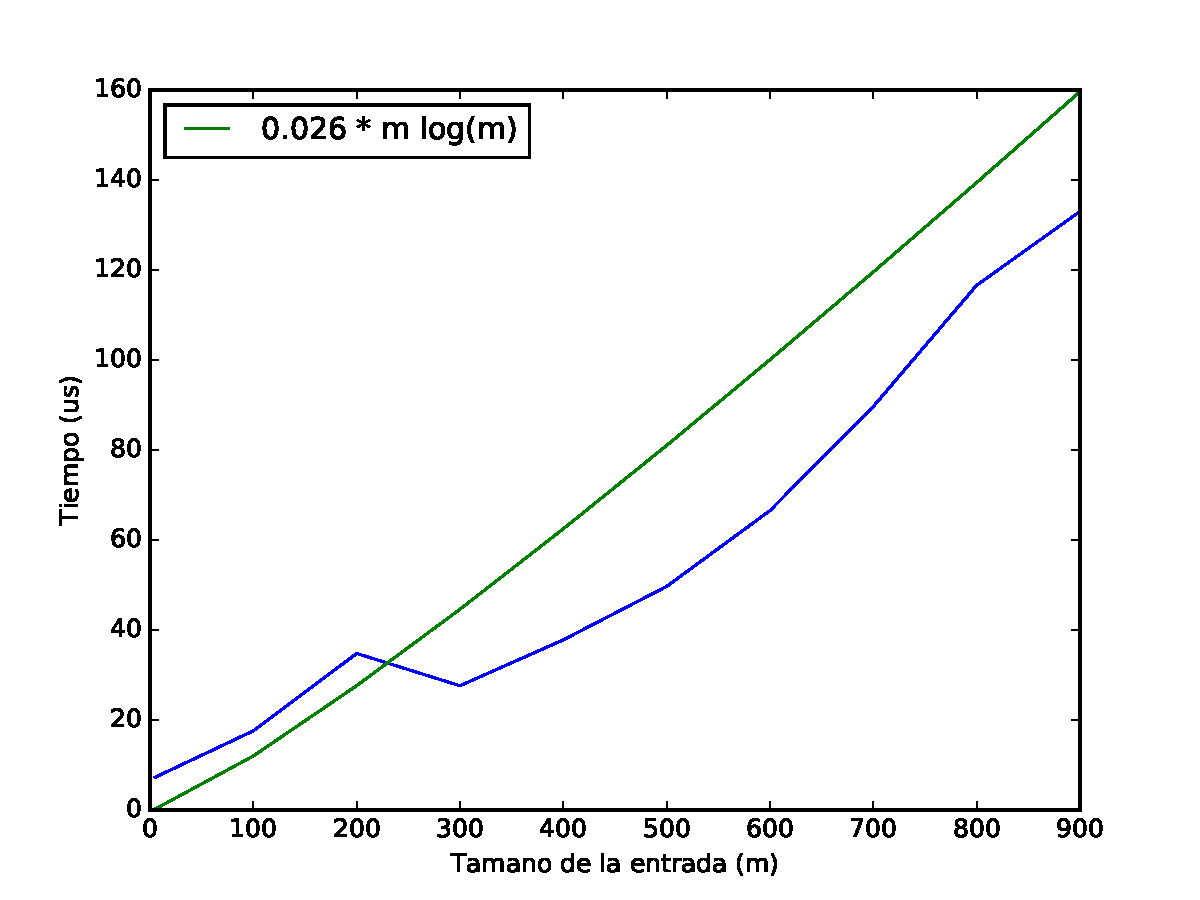
\includegraphics[width=0.8\textwidth]{img/exp/problema2-promedio.pdf}
	\caption{\footnotesize Tiempo que toma el algoritmo en $\mu$s para una entrada de tamaño $m$. $n$ al azar.}
	\label{fig:problema2-promedio}
\end{figure}

\begin{figure}[H]
 \centering
	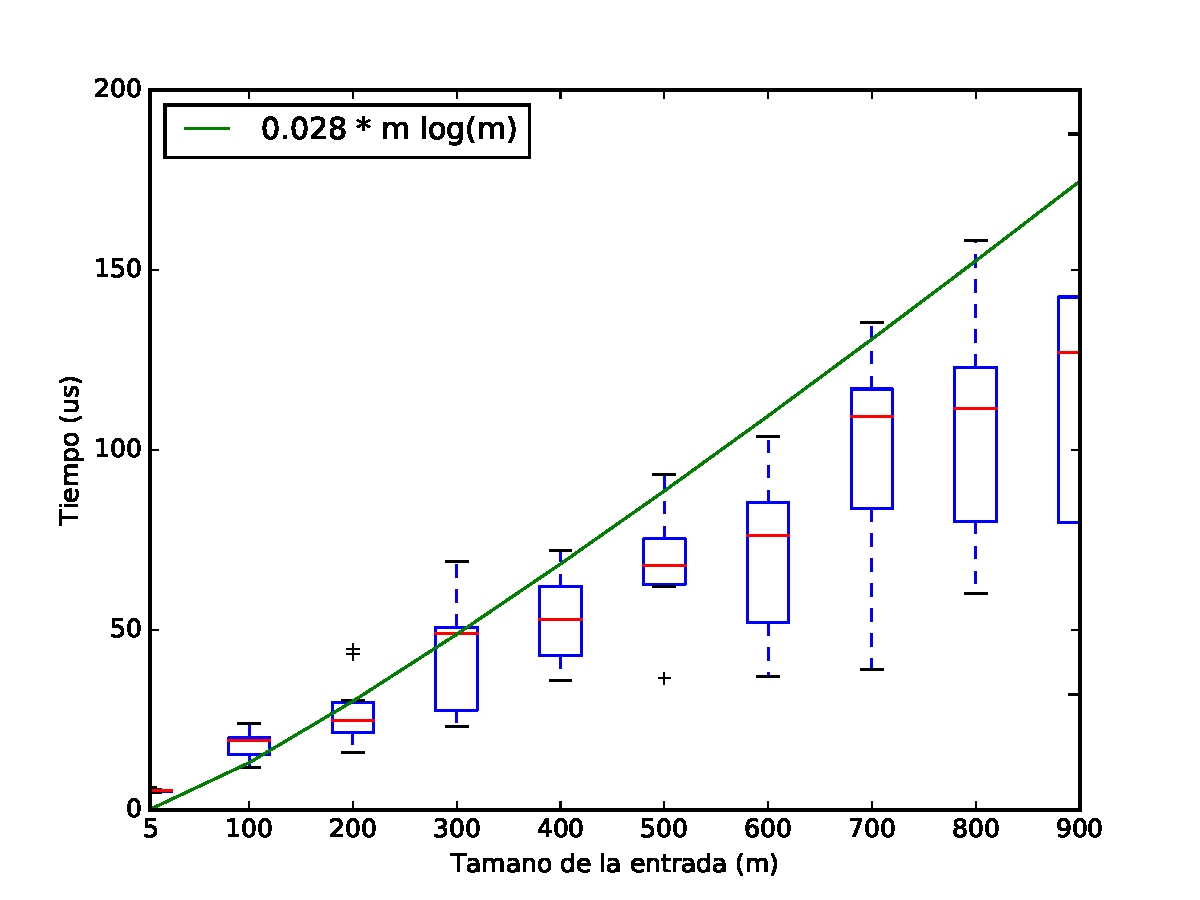
\includegraphics[width=0.8\textwidth]{img/exp/problema2-promedio2.pdf}
  \caption{\footnotesize Tiempo que toma el algoritmo en $\mu$s para una entrada de tamaño $m$. $n$ al azar. Se indican los valores del primer al tercer cuartil con un rectángulo azul y la mediana con una linea roja. El máximo y minimo se indican con lineas negras arriba y abajo del rectángulo.}
	\label{fig:problema2-promedio2}
\end{figure}

\begin{figure}[H]
 \centering
	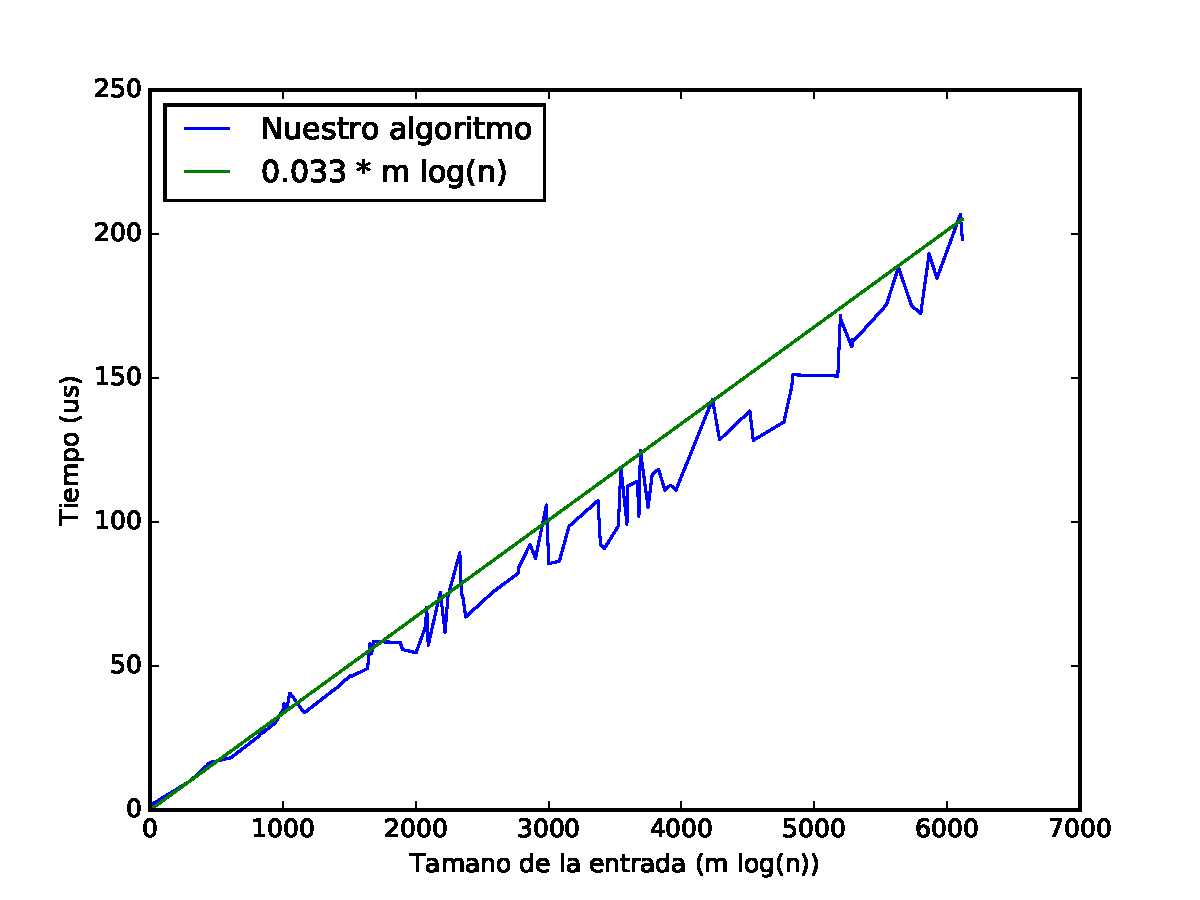
\includegraphics[width=0.8\textwidth]{img/exp/problema2-posta.pdf}
	\caption{\footnotesize Tiempo que toma el algoritmo en $\mu$s para una entrada de tamaño $m \log n$.}
	\label{fig:problema2-posta}
\end{figure}


\subsubsection{M\'etodo de experimentación}

